
\immediate\write18{makeindex \jobname.nlo -s nomencl.ist -o \jobname.nls}

\documentclass[12pt]{ociamthesis}  % default square logo 
%\documentclass[12pt,beltcrest]{ociamthesis} % use old belt crest logo
%\documentclass[12pt,shieldcrest]{ociamthesis} % use older shield crest logo


%load any additional packagessize 
\usepackage{amssymb}
\usepackage{subfigure}

\usepackage{setspace}
\usepackage{array}
\usepackage{float}
\usepackage{algorithm}  
\usepackage{url}
\usepackage{algpseudocode}
\usepackage{graphicx}
\usepackage{wrapfig}
\usepackage{amsmath}
\usepackage{cite}
\usepackage{enumitem}
\usepackage{nomencl}
\makeglossary
\usepackage{emptypage}

\usepackage{fancyhdr}
\usepackage{acronym} 
% \usepackage{tikz} %Not used but is excellent for drawing

\usepackage{afterpage}
\usepackage{lscape}
\usepackage{url}

%---Listing for code----%
\usepackage{listings}

\usepackage{hyperref} % hyperref is the best
\hypersetup{
    colorlinks,
    citecolor=black,
    filecolor=black,
    linkcolor=black,
    urlcolor=black
}
\usepackage[capitalise]{cleveref}
  
\usepackage{color}
\definecolor{gray}{rgb}{0.4,0.4,0.4}
\definecolor{darkblue}{rgb}{0.0,0.0,0.6}
\definecolor{cyan}{rgb}{0.0,0.6,0.6}

\lstset{
  basicstyle=\ttfamily,
  columns=fullflexible,
  showstringspaces=false,
  commentstyle=\color{gray}\upshape
}


\newcommand{\Cov}{\mathrm{Cov}}

%add a new blank page
\newcommand{\newpagenonum}{
  \mbox{}
  \thispagestyle{empty}
  \newpage
}

%vector boldings
\newcommand{\vect}[1]{\mathbf{#1}}


%table captions
\usepackage{caption} 
\captionsetup[table]{skip=5pt}
%input macros (i.e. write your own macros file called mymacros.tex 
%and uncomment the next line)
%\include{mymacros}

\title{Super Amazing Research\\[1ex]     %your thesis title,
         in the Field of Awesomeness}   %note \\[1ex] is a line break in the title

\author{Joe Bloggs}             %your name	
\college{Faculty of Things}  %your college

%\renewcommand{\submittedtext}{change the default text here if needed}
\degree{Doctor of Philosophy}     %the degree
\degreedate{April 2015}         %the degree date
\wordcount{enough}
\makenomenclature

%end the preamble and start the document
\begin{document}
  
%this baselineskip gives sufficient line spacing for an examiner to easily
%markup the thesis with  comments
  % \baselineskip=18pt plus1pt

%set the number of sectioning levels that get number and appear in the contents
\setcounter{secnumdepth}{3}
\setcounter{tocdepth}{3}
\onehalfspacing
% \doublespacing


\maketitle                 			 % create a title page from the preamble info
\cleardoublepage  
\begin{romanpages_onepage}     	    							      % start roman page numbering
  \begin{abstractlong}
\begin{singlespace}
\noindent This thesis investigates ....

\end{singlespace}
\end{abstractlong}
% \newpagenonum          				% include the abstracttwo 
	\begin{dedication2}
\noindent This thesis is dedicated to Tom Kent,\\
for making this amazing template!
\end{dedication2}
% \newpagenonum
      				% include a dedication.tex file
	\begin{acknowledgementslong}
%Arthur
I would like to begin by expressing my profound gratitude and appreciation to Tom Kent for making this sweet template.

Also probably the oclaim template it is based on, although I can no longer find the repo on github.


\end{acknowledgementslong}
\newpagenonum 	% include an acknowledgements.tex file
	\begin{declarationlong}
% Thesis Abstract -----------------------------------------------------


%\begin{declarationlong}    %uncommenting this line, gives a different abstract heading
%\begin{declaration}        %this creates the heading for the abstract page

%\chapter*{Author's Declaration}
%\begin{spacing}{1.0}
\noindent I declare that the work in this dissertation was carried out in accordance with the requirements of the University's Regulations and Code of Practice for Research Degree Programmes and that it has not been submitted for any other academic award. Except where indicated by specific reference in the text, the work is the candidate's own work. Work done in collaboration with, or with the assistance of, others, is indicated as such. Any views expressed in the dissertation are those of the author.
%\end{spacing}

\vspace{25 mm}
% \textbf{\large{Signed .............................................................}}
\textbf{\large{Signed}}
\vspace{15 mm}

% \textbf{\large{Date    ..........................}}
\textbf{\large{Date}}
% \vspace{10 mm}
% \textbf{\large{DATE:}}


%SIGNED: .............................................................  DATE:..........................


%\end{declaration}
%\end{declarationlong}


% ----------------------------------------------------------------------


%%% Local Variables: 
%%% mode: latex
%%% TeX-master: "../thesis"
%%% End: 

\end{declarationlong}
\mbox{}
\thispagestyle{empty}
% \newpagenonum 		 	  	% include debclaration to sign
			% Make the nomenclature	
	\printnomenclature[2.5 cm] 
  \chapter*{Acronyms}
\begin{acronym}[ZFTOWW]
	\acro{ATAG}{Air Transport Action Group}

	\acro{ATC}{Air Traffic Control}

	\acro{BADA}{Base of Aircraft Data}
	\acro{BL}{Bottom Left}
	\acro{BR}{Bottom Right}

	\acro{CI}{Confidence Interval}
	\acro{CSV}{Comma Separated Values}

	\acro{DP}{Dynamic Programming}

	\acro{EAM}{Estimated Assignment Method}

	\acro{GC}{Geometric Cost}
	\acro{GR}{Geometric Routing}	
	\acro{GUI}{Graphical User Interface}

	\acro{HGV}{Heavy Goods Vehicle}
	\acro{HPC}{High Performance Computer}

	\acro{JS}{Jet Stream}

	\acro{KML}{Keyhole Markup Language}

	\acro{MILP}{Mixed Integer Linear Program}

	\acro{NAT}{North Atlantic Tracks}
	\acro{NBD}{Negative Binomial Distribution}
	\acro{NTP}{No Takeoff Policy}

	\acro{OAG}{Official Airline Guide}
	\acro{OSM}{Open Street Map}

	\acro{PDF}{Probability Density Function}

	\acro{SDP}{Stochastic Dynamic Programming}

	\acro{TR}{Top Right}
	\acro{TL}{Top Left}

	\acro{VI}{Value Iteration}

	\acro{WR}{Wind Routing}
	\acro{WC}{Wind Cost}

	\acro{ZFTOW}{Zero Fuel Take Off Weight}


\end{acronym}         %include the acronyms
	\tableofcontents         	   % generate and include a table of contents
	\listoffigures            	  % generate and include a list of figures
  \listoftables
  \cleardoublepage
\end{romanpages_onepage}            % end roman page numbering


% now include the files of latex for each of the chapters etc
% each chapter should be in its own folder:
% ../ChapterN
% ../ChapterN/figures/
% this keeps things clean, and means you can comment out chapters to speed up compilation!
\chapter{Introduction}\label{chapter:1}

%------------------------------------------------------------%
%------------ Introduction to The Field/Context -------------%
%------------------------------------------------------------%

\section{Formation Flight}
	Scientist have long looked to nature for inspiration; the field of biomimicry is devoted to developing techniques to emulate nature's strategies. One motivating example is how geese, and other migratory birds, fly in a `V' formation \cite{Gould1974,Hainsworth1989,Cutts1994,Weimerskirch2001,Portugal2014} when travelling long distances. Key research shows that birds participating in such formations will have significant increases to their range \cite{Lissaman1970,Cutts1994} while exhibiting lower heart rates \cite{Weimerskirch2001} during flight compared to flying alone. 


		\begin{figure}[ht]
		\centering
		\subfigure[Top-Down View]{
		\includegraphics[width= 0.65 \columnwidth]{Chapter01/figures/wake-vortex-top.eps}
		\label{fig:vortex-top}
		}
		\subfigure[Rear view]{
		\includegraphics[width= 0.65 \columnwidth]{Chapter01/figures/wake-vortex-rear.eps}
		\label{fig:vortex-rear}
		}
		\caption[Wing-tip vortices and regions of upwash and downwash]{Wing-tip vortices and regions of upwash and downwash}\label{fig:vortices}
		\end{figure}

	The aerodynamic fundamentals behind formation flight for aircraft are fairly well studied \cite{Okolo2014,Pahle2012,Ning2011,Liu2015,Blake2004a}. As an aircraft flies, the pressure differentials created over the wings' surface, generates lift. The wake left behind the lifting-wing induces downwash inboard, between the aircraft wingtips, and a corresponding upwash outboard as depicted in \Cref{fig:vortices}. A trailing aircraft flying through this region of upwash can maintain its flight while operating at a lower apparent angle of attack, that is, a lower angle of attack relative to the horizon. Therefore the aircraft observes a significant reduction in induced drag and as a result a corresponding reduction in fuel burn. 





\chapter{A Geometric Method for Optimal Formation Flight Routes}\label{chp:2}


\section{Introduction}

	Hello.
 
\chapter{Wind-optimal Routing for Formation Flight}\label{chp:3}



	\section{Wind Routing Method}\label{sec:wind_method}	
		While weather is chaotic and difficult to accurately predict over longer periods of time, short term `day-to-day' weather forecasts are generally easier to predict. Aircraft flight plans, chosen prior to takeoff account for a wide variety of both predictable and unpredictable factors. This typically includes the use of weather forecasts to avoid potentially adverse weather ....

		\subsection{Generating Static Wind Fields}\label{sec:wind_fields}
			To generate wind fields, a set of evenly spaced geographical points is first generated across the entire map. Each of these points are then assigned vectors with a random direction and a random (but bounded) magnitude. 
			...
				\begin{figure}[ht]
				\centering
					\subfigure[Low volatility]
					{
					\frame{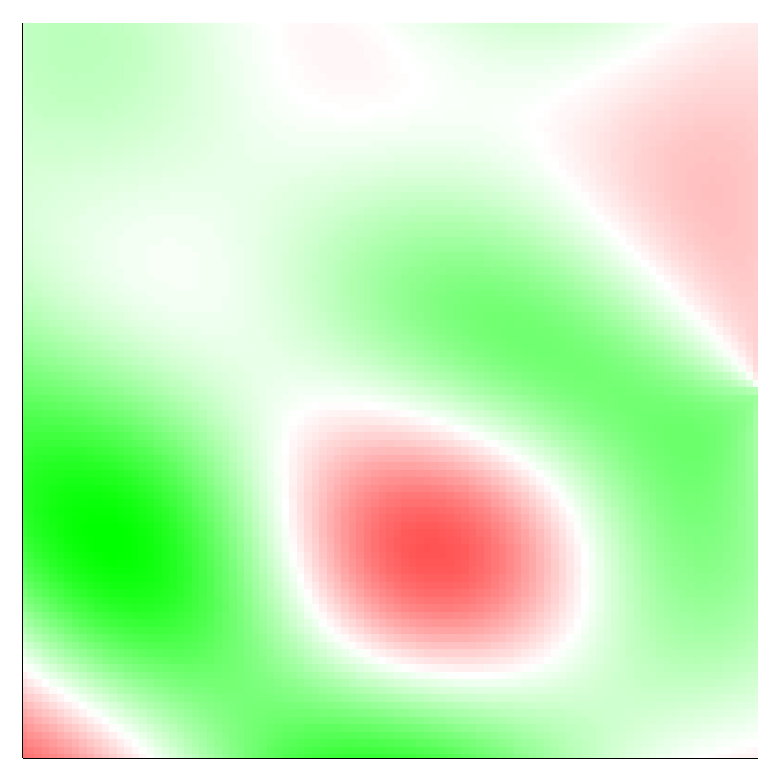
\includegraphics[width= 0.3 \columnwidth]{Chapter03/figures/Wind_plot_r1}}
					}
					\subfigure[Medium volatility]
					{
					\frame{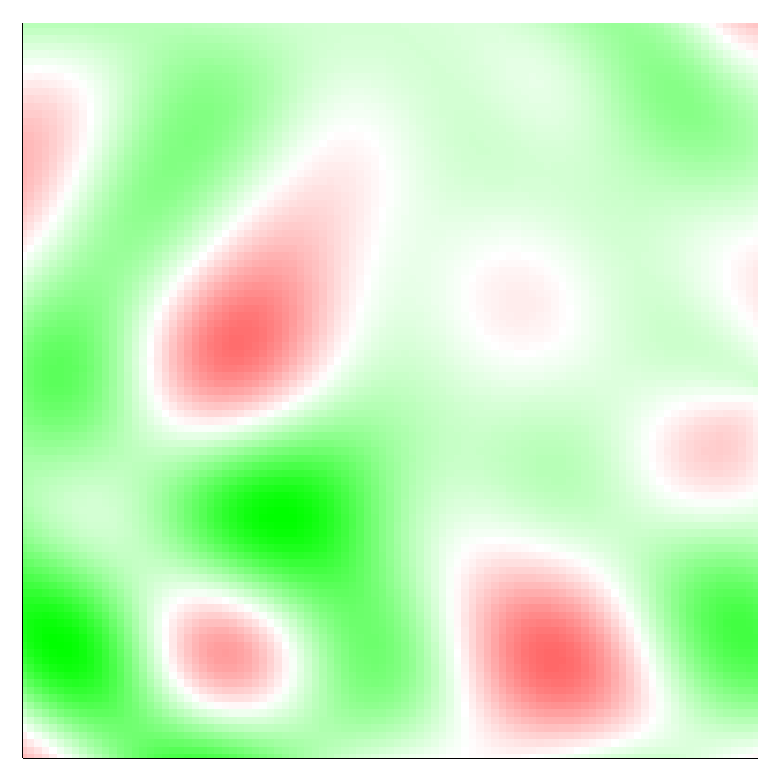
\includegraphics[width= 0.3 \columnwidth]{Chapter03/figures/Wind_plot_r2}}
					}
					\subfigure[High volatility]
					{
					\frame{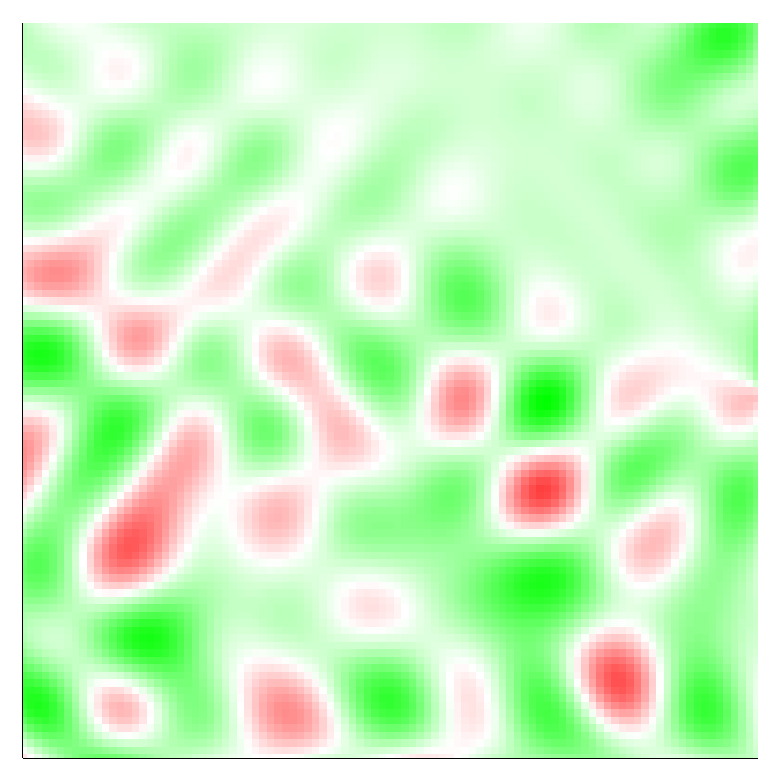
\includegraphics[width= 0.3 \columnwidth]{Chapter03/figures/Wind_plot_r4}}
					}
				\caption{Random wind fields for different levels of volatility}
					\label{fig:windfields}
				\end{figure}

		

		\input{Chapter03/Results-CS.dat}%results from casestudy variables
		\input{Chapter03/Results-CS-Est.dat}%using the Estimated Assignment method
		\input{Chapter03/Results-EAM-changes.dat}%using the Estimated Assignment method

		 \subsection{Jet-Stream West-to-East}\label{sec:WE}
		 	The formation results travelling from West-to-East over the Atlantic, with a wind field representational of the Jet-Stream, are now shown. 
		 	...

		 	results in a globally optimal solution. The resulting assignment equates to a saving of roughly \ValWindpcWE$\%$, against the corresponding solo flights routed through wind, and takes around 180 hours. This runtime break down as follows:
			\begin{samepage}
		 	\begin{description}
			 	\item[Enumeration: Solo] 210 solo flights routed for wind: 10 minutes;
			 	\item[Enumeration: Formations] 21,945 formations routed for wind: 180 hours; 
			 	\item[Assignment] MILP assignment: 4 seconds; 
			 	\item[Post-Process] None;
			 	\item[Total] 180 hours.
		 	\end{description}
		 	\end{samepage}

	 	 	A proportion of the saving achieved comes from cruising with a tailwind, so makes any possible saving clearly dependent on the particular wind field used. The routes of this solution are shown in ...

		 	If instead Method 2 is used, where the enumeration stage is done using geometric routing and then using these costs an assignment is made,  

		 	... 

		 	The resulting assignment, when routed through wind, achieves \ValGeoWindpcWE$\%$ against solo flight, but takes significantly less time at around 60 minutes. This runtime breaks down as follows: 
			\begin{samepage}
		 	\begin{description}
			 	\item[Enumeration: Formations] 21,945 formations routed geometrically: 10 seconds; 
			 	\item[Assignment] MILP assignment: 4 seconds; 
			 	\item[Post-Process: Solo] 210 solo flights routed for wind: 10 minutes.
			 	\item[Post-Process: Formations] 105 assigned formations routed for wind: 50 minutes.
			 	\item[Total] 60 minutes
		 	\end{description}
		 	\end{samepage}
		 	The geometric assignment routed through wind is plotted ... only \ValSameFormWE\ formation pairs, roughly \ValSameFormpcWE\%, remain the same between the two assignments.
		 	
		






\include{Conclusion/Conclusion}

%now enable appendix numbering format and include any appendices
\appendix
% \include{Appendices/Appendix1}
% \include{Appendices/Appendix2}

%next line adds the Bibliography to the contents page
\addcontentsline{toc}{chapter}{Bibliography}
%uncomment next line to change bibliography name to references\useexternalfile{
%\renewcommand{\bibname}{References}
\bibliography{library}      %use a bibtex bibliography file refs.bib
% \bibliographystyle{IEEEtran}   %use the plain bibliography style
\bibliographystyle{ieeetr}   %use the plain bibliography style
\end{document}

